%%%%%%%%%%%%%%%%%%%%%%%%%%%%%%%%%%%%%%%%%%%%%%%%%%%%%%%%%%%%%%%%%%%%%%
% How to use writeLaTeX: 
%
% You edit the source code here on the left, and the preview on the
% right shows you the result within a few seconds.
%
% Bookmark this page and share the URL with your co-authors. They can
% edit at the same time!
%
% You can upload figures, bibliographies, custom classes and
% styles using the files menu.
%
%%%%%%%%%%%%%%%%%%%%%%%%%%%%%%%%%%%%%%%%%%%%%%%%%%%%%%%%%%%%%%%%%%%%%%

\documentclass[12pt]{article}

\usepackage{sbc-template}

\usepackage{graphicx,url}

%\usepackage[brazil]{babel}   
\usepackage[utf8]{inputenc} 

\usepackage{float}
\usepackage{hyperref}
     
\sloppy

\title{Semáforo de Carros + Pedestre}

\author{Fabricio Araújo Dias}

\address{Instituto Federal de Educação, Ciência e Tecnologia do Ceará
  (IFCE)\\
  Avenida Vice-Presidente José Alencar, S/N -- 61.939-140 -- Maracanaú -- CE -- Brasil
  \email{fabricio.araujo61@aluno.ifce.edu.br}
}

\begin{document} 

\maketitle

\begin{abstract}
  This report describes the step-by-step practical activity for the Microcontrollers course, which consists of implementing a traffic light for cars and pedestrians using two LEDs and a button. The logic for running the traffic light was defined, but the configuration on the ESP32 was partial - the button pin had yet to be connected.
\end{abstract}
     
\begin{resumo} 
  Esse relatório descreve o passo a passo da atividade prática da disciplina de Microcontroladores que consiste em implementar um semáforo para carros e pedestres utilizando dois LEDS e um botão. A lógica para o funcionamento do semáforo foi definida, mas a configuração no ESP32 foi parcial - faltando a ligação do pino do botão.
\end{resumo}


\section{Introdução}\label{sec:introdução}
A segunda atividade prática foi uma configuração de dois LEDS RGB para que eles funcionem como um semáforo de carro e pedestre. Quando se aperta um botão, há um tempo de espera antes que os semáforos se alterem.

\section{Desenvolvimento do Código}\label{sec:desenvolvimento-do-código}

Primeiro, foi definido constantes para representar o número dos pinos para a realização do semáforo. Os pinos para o semáforo dos carros foram 21, 22 e 23 para vermelho, verde e azul, respectivamente. Já os pinos para o semáforo dos pedestres foram 33, 32 e 26 para vermelho, verde e azul, respectivamente. A cor azul é usada no lugar da cor amarela.

Também foi definido o pino para o botão que os pedestres irão pressionar que foi o pino 19.

Por fim, foi definido o tempo de espera para os carros esperarem enquanto o sinal está vermelho e o tempo de atenção para a mudança de cor do semáforo.

Em setup, a grande maioria dos modos dos pinos foram configurados para saída (OUTPUT), com exceção apenas do pino para o botão que foi configurado para entrada. Por fim, colocamos para que não passe tensão para o pino do botão.

Separamos o problema em quatro situações: o sinal de trânsito está verde e o sinal de pedestre está vermelho; o sinal de trânsito está azul e o sinal de pedestre está vermelho; o sinal de trânsito está vermelho e o sinal de pedestre está verde; e o sinal de trânsito está vermelho e o sinal de pedestre está azul.

Transformamos essas situações em funções para uma melhor organização. Cada função irá indicar se em tal pino ocorrerá tensão ou não para a luz desejada no momento utilizando a função digitalWrite. Mesmo que algumas diretivas sejam desnecessárias, elas foram mantidas para em caso de futuras alterações a cor escolhida não sofra alterações.

As funções são: carRun; carAttention; pedestrianRun; e pedestrianAttention. Excluindo carRun, as funções possuem um tempo de espera no final das diretivas antes que ele se encerre e vá para a próxima função. Para as funções "Attention", o tempo de espera é de 2 segundos, e para a função pedestrianRun, o tempo de espera é de 5 segundos. A função carRun não possui tempo de espera, pois ela é a função padrão a ser executada, e se supõe que o semáforo não é de um cruzamento.

Por fim, a questão de apertar o botão para o sinal fechar foi feita utilizando um condicional para conferir se está passando tensão pelo pino do botão utilizando a função DigitalRead. Se estiver passando, é que alguém pressionou o botão, então o fluxo irá entrar para o condicional que possui as funções carAttention, pedestrianRun e pedestrianAttention. Caso não esteja passando tensão, a função carRun será executada.

O código pode ser conferido nesse \href{https://github.com/fabricio-araujo94/microcontroladores/tree/main/semaforo}{repositório no Github}.

\section{Configuração no ESP32}\label{sec:configuração-no-esp32}

Como foi especificado na seção do código, os pinos para o LED do semáforo de carros foram os pinos 21, 22 e 23; e os pinos para o LED do semáforo dos pedestres foram os pinos 33, 32 e 26. Com os LEDS posicionados na protoboard, para cada terminal é conectado um resistor de 390 ohms para então conectar o cabo macho referente ao pino. O cátodo é conectado à GND e não se utilizou um resistor.

O botão foi posicionado na protoboard para que os pares de terminais fiquem em colunas diferentes. Foi conectado o pino 19 ao terminal positivo na protoboard. O terminal negativo foi ligado à GND sem antes passar por um resistor. A questão do resistor no terminal negativo garante que não está passando tensão pela entrada. Sem ele, o botão ainda funcionará, mas corre um risco dele ser acionado inesperadamente.

\section{Considerações Finais}\label{sec:considerações-finais}

\begin{figure}[H]
    \centering
    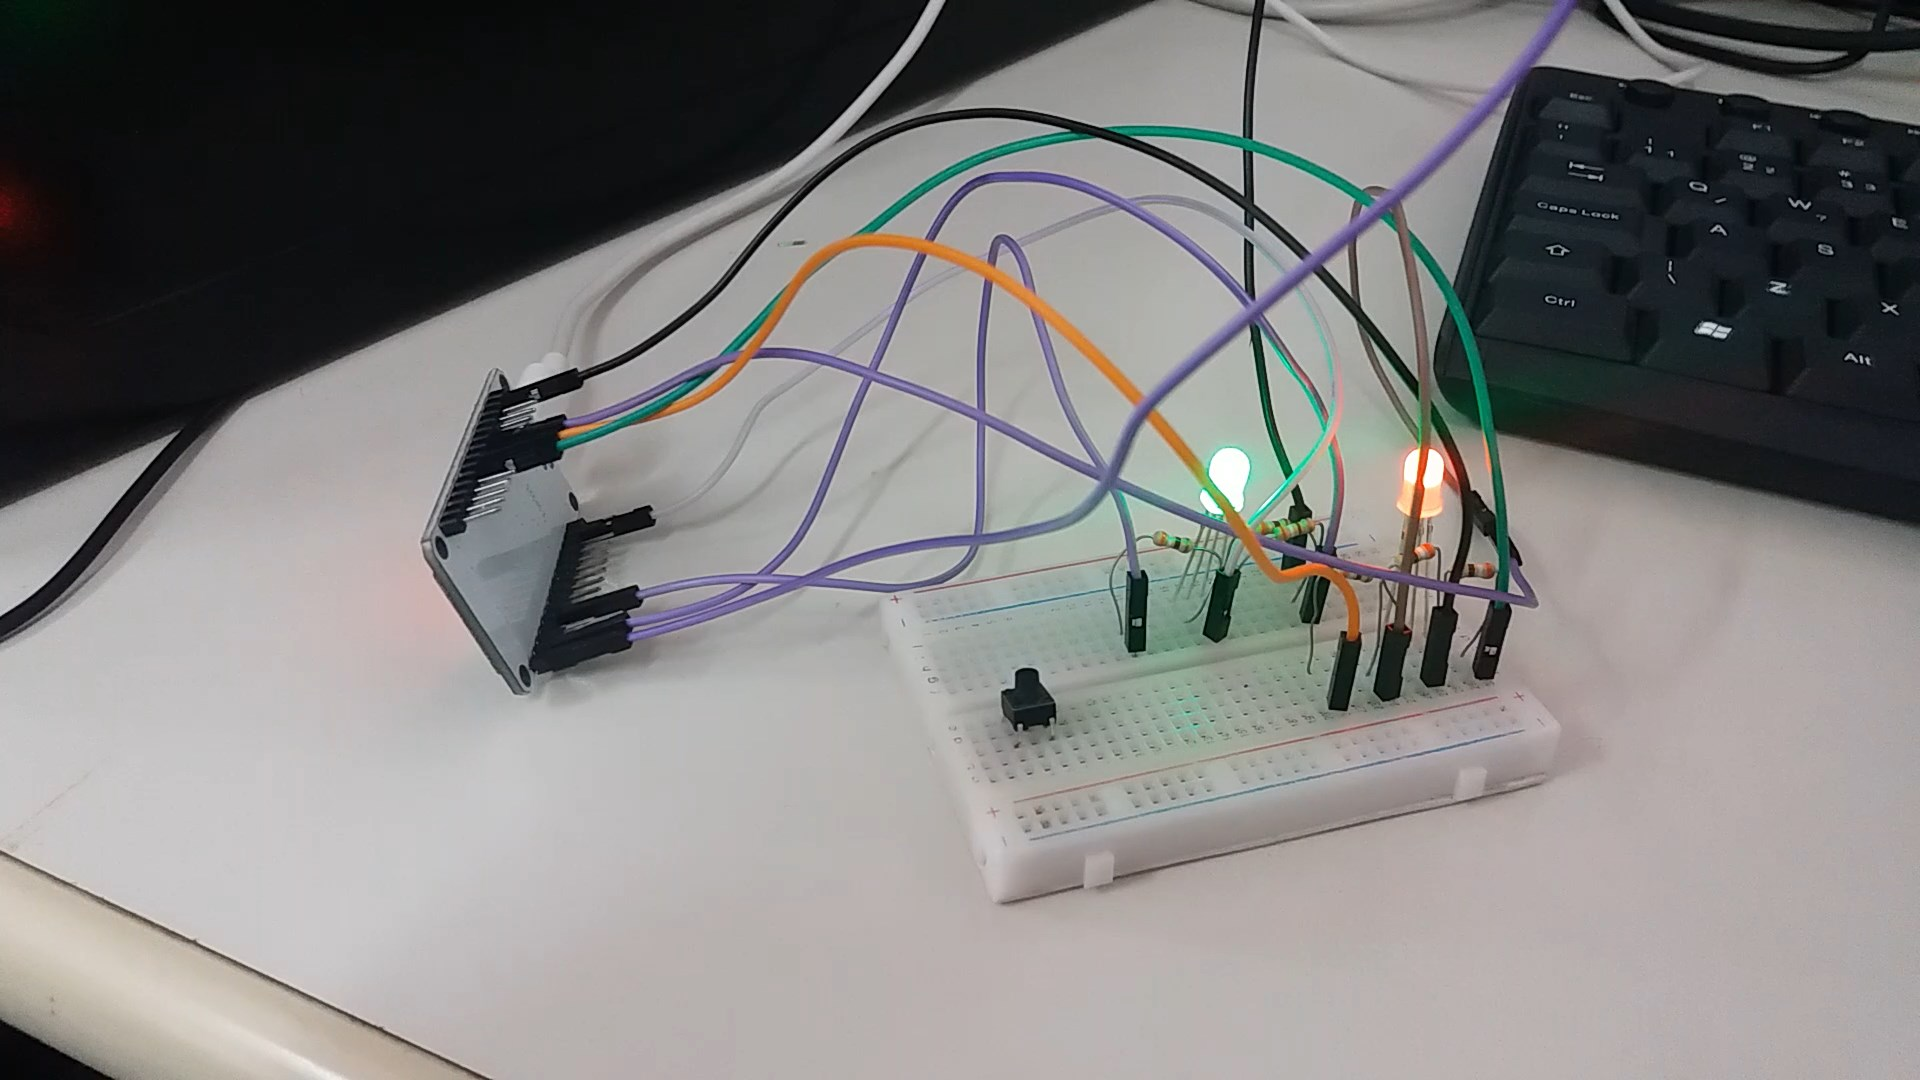
\includegraphics[width=0.5\linewidth]{img/20241030_094251.mp4_snapshot_00.01.049.jpg}
    \caption{Configuração parcial na protoboard}
    \label{fig:protoboard}
\end{figure}

Feito tudo isso, o semáforo de carros e pedestres estará funcionando. Não restou tempo para ligar os pinos do botão durante a prática na sala de aula. A ligação dos pinos do botão foi testada no simulador online Wokwi. É possível conferir o resultado parcial nesse \href{https://youtu.be/4dnnWBfyLOo}{vídeo no Youtube}. Para testar, o semáforo dos carros fecha a cada 7 segundos.


\end{document}
